% Options for packages loaded elsewhere
\PassOptionsToPackage{unicode}{hyperref}
\PassOptionsToPackage{hyphens}{url}
%
\documentclass[
  english,
  man]{apa6}
\author{\phantom{0}}
\date{}

\usepackage{amsmath,amssymb}
\usepackage{lmodern}
\usepackage{iftex}
\ifPDFTeX
  \usepackage[T1]{fontenc}
  \usepackage[utf8]{inputenc}
  \usepackage{textcomp} % provide euro and other symbols
\else % if luatex or xetex
  \usepackage{unicode-math}
  \defaultfontfeatures{Scale=MatchLowercase}
  \defaultfontfeatures[\rmfamily]{Ligatures=TeX,Scale=1}
\fi
% Use upquote if available, for straight quotes in verbatim environments
\IfFileExists{upquote.sty}{\usepackage{upquote}}{}
\IfFileExists{microtype.sty}{% use microtype if available
  \usepackage[]{microtype}
  \UseMicrotypeSet[protrusion]{basicmath} % disable protrusion for tt fonts
}{}
\makeatletter
\@ifundefined{KOMAClassName}{% if non-KOMA class
  \IfFileExists{parskip.sty}{%
    \usepackage{parskip}
  }{% else
    \setlength{\parindent}{0pt}
    \setlength{\parskip}{6pt plus 2pt minus 1pt}}
}{% if KOMA class
  \KOMAoptions{parskip=half}}
\makeatother
\usepackage{xcolor}
\IfFileExists{xurl.sty}{\usepackage{xurl}}{} % add URL line breaks if available
\IfFileExists{bookmark.sty}{\usepackage{bookmark}}{\usepackage{hyperref}}
\hypersetup{
  pdflang={en-EN},
  hidelinks,
  pdfcreator={LaTeX via pandoc}}
\urlstyle{same} % disable monospaced font for URLs
\usepackage{longtable,booktabs,array}
\usepackage{calc} % for calculating minipage widths
% Correct order of tables after \paragraph or \subparagraph
\usepackage{etoolbox}
\makeatletter
\patchcmd\longtable{\par}{\if@noskipsec\mbox{}\fi\par}{}{}
\makeatother
% Allow footnotes in longtable head/foot
\IfFileExists{footnotehyper.sty}{\usepackage{footnotehyper}}{\usepackage{footnote}}
\makesavenoteenv{longtable}
\usepackage{graphicx}
\makeatletter
\def\maxwidth{\ifdim\Gin@nat@width>\linewidth\linewidth\else\Gin@nat@width\fi}
\def\maxheight{\ifdim\Gin@nat@height>\textheight\textheight\else\Gin@nat@height\fi}
\makeatother
% Scale images if necessary, so that they will not overflow the page
% margins by default, and it is still possible to overwrite the defaults
% using explicit options in \includegraphics[width, height, ...]{}
\setkeys{Gin}{width=\maxwidth,height=\maxheight,keepaspectratio}
% Set default figure placement to htbp
\makeatletter
\def\fps@figure{htbp}
\makeatother
\setlength{\emergencystretch}{3em} % prevent overfull lines
\providecommand{\tightlist}{%
  \setlength{\itemsep}{0pt}\setlength{\parskip}{0pt}}
\setcounter{secnumdepth}{-\maxdimen} % remove section numbering
% Make \paragraph and \subparagraph free-standing
\ifx\paragraph\undefined\else
  \let\oldparagraph\paragraph
  \renewcommand{\paragraph}[1]{\oldparagraph{#1}\mbox{}}
\fi
\ifx\subparagraph\undefined\else
  \let\oldsubparagraph\subparagraph
  \renewcommand{\subparagraph}[1]{\oldsubparagraph{#1}\mbox{}}
\fi
% Manuscript styling
\usepackage{upgreek}
\captionsetup{font=singlespacing,justification=justified}

% Table formatting
\usepackage{longtable}
\usepackage{lscape}
% \usepackage[counterclockwise]{rotating}   % Landscape page setup for large tables
\usepackage{multirow}		% Table styling
\usepackage{tabularx}		% Control Column width
\usepackage[flushleft]{threeparttable}	% Allows for three part tables with a specified notes section
\usepackage{threeparttablex}            % Lets threeparttable work with longtable

% Create new environments so endfloat can handle them
% \newenvironment{ltable}
%   {\begin{landscape}\centering\begin{threeparttable}}
%   {\end{threeparttable}\end{landscape}}
\newenvironment{lltable}{\begin{landscape}\centering\begin{ThreePartTable}}{\end{ThreePartTable}\end{landscape}}

% Enables adjusting longtable caption width to table width
% Solution found at http://golatex.de/longtable-mit-caption-so-breit-wie-die-tabelle-t15767.html
\makeatletter
\newcommand\LastLTentrywidth{1em}
\newlength\longtablewidth
\setlength{\longtablewidth}{1in}
\newcommand{\getlongtablewidth}{\begingroup \ifcsname LT@\roman{LT@tables}\endcsname \global\longtablewidth=0pt \renewcommand{\LT@entry}[2]{\global\advance\longtablewidth by ##2\relax\gdef\LastLTentrywidth{##2}}\@nameuse{LT@\roman{LT@tables}} \fi \endgroup}

% \setlength{\parindent}{0.5in}
% \setlength{\parskip}{0pt plus 0pt minus 0pt}

% \usepackage{etoolbox}
\makeatletter
\patchcmd{\HyOrg@maketitle}
  {\section{\normalfont\normalsize\abstractname}}
  {\section*{\normalfont\normalsize\abstractname}}
  {}{\typeout{Failed to patch abstract.}}
\patchcmd{\HyOrg@maketitle}
  {\section{\protect\normalfont{\@title}}}
  {\section*{\protect\normalfont{\@title}}}
  {}{\typeout{Failed to patch title.}}
\makeatother
\shorttitle{SHORTTITLE}
\usepackage{csquotes}
\usepackage{float}
\usepackage{sectsty}
\usepackage{lscape}
\newcommand{\blandscape}{\begin{landscape}}
\newcommand{\elandscape}{\end{landscape}}
\ifXeTeX
  % Load polyglossia as late as possible: uses bidi with RTL langages (e.g. Hebrew, Arabic)
  \usepackage{polyglossia}
  \setmainlanguage[]{english}
\else
  \usepackage[main=english]{babel}
% get rid of language-specific shorthands (see #6817):
\let\LanguageShortHands\languageshorthands
\def\languageshorthands#1{}
\fi
\ifLuaTeX
  \usepackage{selnolig}  % disable illegal ligatures
\fi


\affiliation{\phantom{0}}

\begin{document}

\hypertarget{chapitre-3-utiliser-lanova-bf-emph-w-de-welch-par-duxe9faut}{%
\section{\texorpdfstring{Chapitre 3 : Utiliser l'ANOVA \(\bf \emph W\) de Welch par défaut}{Chapitre 3 : Utiliser l'ANOVA \textbackslash bf \textbackslash emph W de Welch par défaut}}\label{chapitre-3-utiliser-lanova-bf-emph-w-de-welch-par-duxe9faut}}

\begin{center}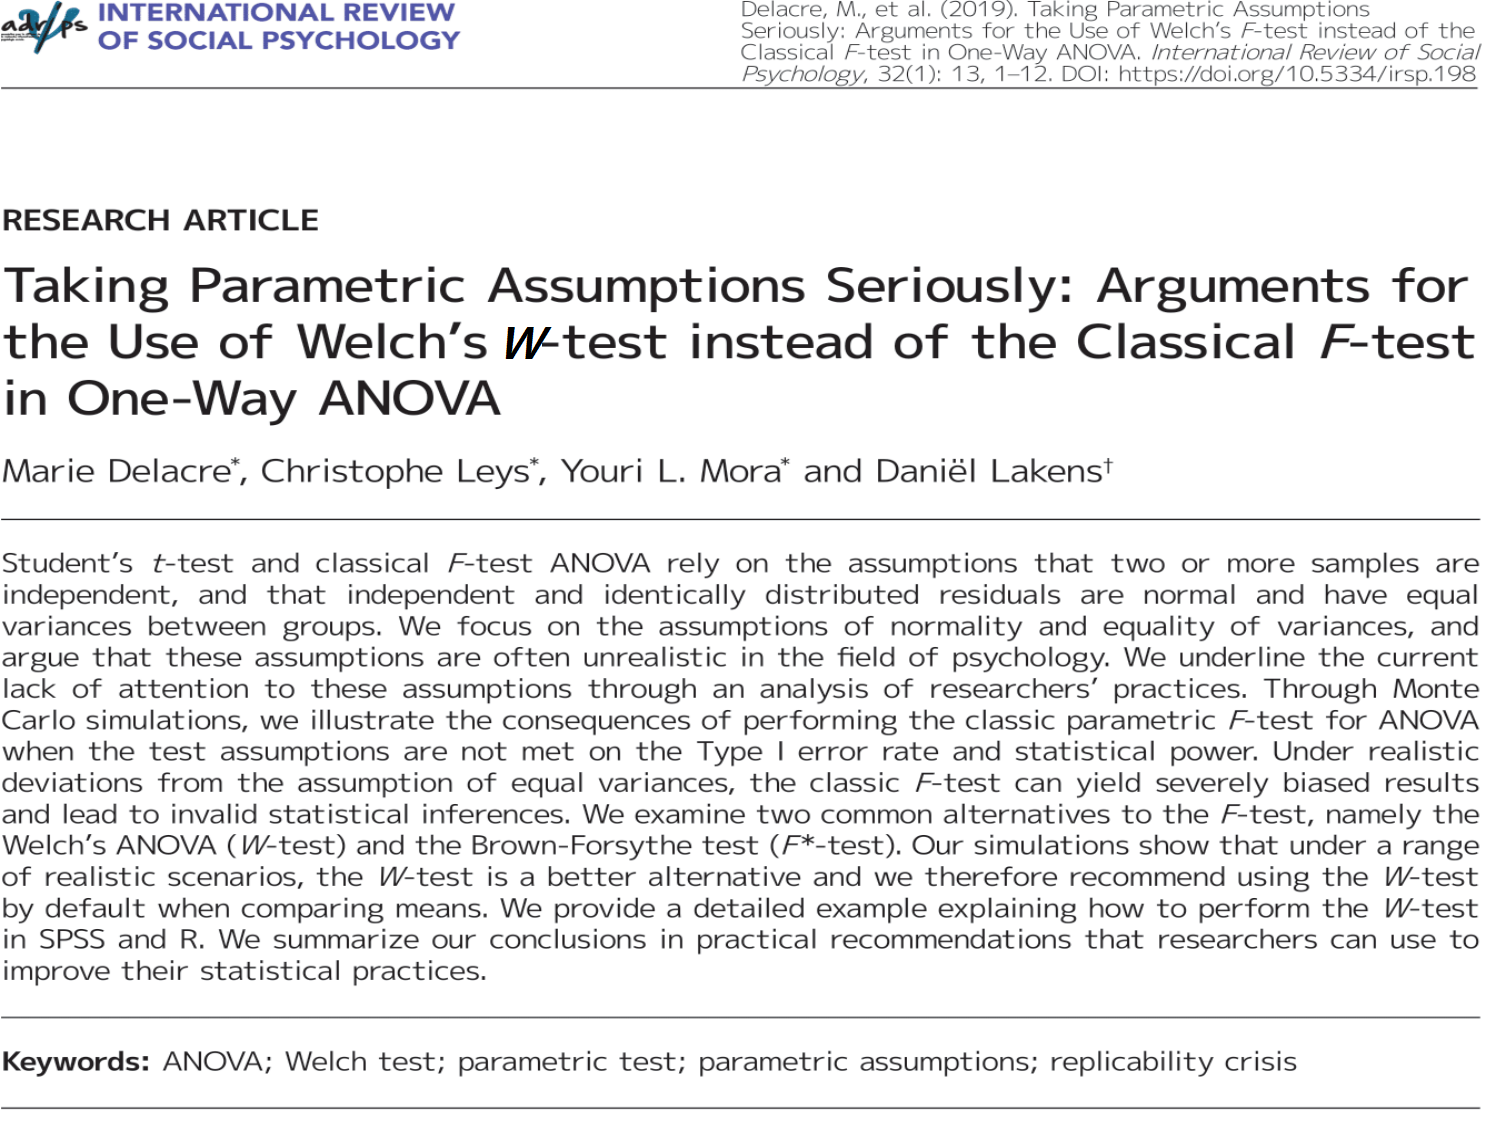
\includegraphics[height=0.54\textheight]{C:/Users/mdelacre/Documents/Github project/thesis/Chapitre 3/Chapitre 3-couverture} \end{center}

When comparing independent groups researchers often analyze the means by performing a Student's \emph{t}-test or classical Analysis of Variance (ANOVA) \emph{F}-test (\textbf{erceg-hurn\_modern\_2008?}; \textbf{keselman\_statistical\_1998?}; \textbf{Tomarken\_and\_Serlin\_1986?}). Both tests rely on the assumptions that independent and identically distributed residuals (1) are sampled from a normal distribution and (2) have equal variances between groups (or homoscedasticity; see \textbf{Lix\_Keselman\_Keselman\_1996?}). While a deviation from the normality assumption generally does not strongly affect either the Type I error rates (Glass et al., 1972; Harwell et al., 1992; Tiku, 1971) or the power of the \emph{F}-test (\textbf{Harwell\_et\_al\_1992?}; \textbf{David\_and\_Johnson\_1951?}; \textbf{Srivastava\_1959?}; \textbf{tiku\_power\_1971?}), the \emph{F}-test is not robust against unequal variances (\textbf{grissom\_heterogeneity\_2000?}). Unequal variances can alter both the Type I error rate (David \(\&\) Johnson, 1951; Harwell et al., 1992) and statistical power (Nimon, 2012; Overall et al., 1995) of the \emph{F}-test.

Although it important to make sure test assumptions are met before a statistical test is performed, researchers rarely provide information about test assumptions when they report an \emph{F}-test. We examined statistical tests reported in 116 articles in the \emph{Journal of Personality and Social Psychology} published in 2016. Fourteen percent of these articles reported a one-way \emph{F}-test, but only one article indicated that the homogeneity of variances assumption was taken into account. They reported corrected degrees of freedom for unequal variances, which could signal the use of the \emph{W}-test instead of the classical \emph{F}-test. A similar investigation (Hoekstra et al., 2012) yielded conclusions about the lack of attention to both the homoscedasticity and the normality assumptions. Despite the fact that the \emph{F}-test is currently used by default, better alternatives exist, such as the Welch's \emph{W} ANOVA (\emph{W}-test), the Alexander-Govern test, James' second order test, and the Brown-Forsythe ANOVA (\emph{F}*-test). Although not the focus of the current article, additional tests exist that allow researchers to compare groups either based on other estimators of central tendency than the mean (see for example \textbf{erceg-hurn\_modern\_2008?}; \textbf{wilcox\_how\_1998?}), or based on other relevant parameters of distribution than the central tendency, such as standard deviations and the shape of the distribution (\textbf{grissom\_heterogeneity\_2000?}; \textbf{Tomarken\_and\_Serlin\_1986?}). However, since most researchers currently generate hypotheses about differences between means (\textbf{erceg-hurn\_modern\_2008?}; \textbf{keselman\_statistical\_1998?}), we think that a realistic first step towards progress would be to get researchers to correctly test the hypothesis they are used to.

Although the debate surrounding the assumptions of the \emph{F}-test has been widely explored (see for example the meta-analysis of Harwell et al., 1992), applied researchers still largely ignore the consequences of assumption violations. Non-mathematical pedagogical papers summarizing the arguments seem to be lacking from the literature, and the current paper aims to fill this gap. We will discuss the pertinence of the assumptions of the \emph{F}-test, and focus on the question of heteroscedasticity (that, as we will see, can have major consequences on error rates). We will provide a non-mathematical explanation of how alternatives to the classical \emph{F}-test cope with heteroscedasticity violations. We conducted simulations in which we compare the \emph{F}-test with the most promising alternatives. We argue that when variances are equal between groups, the \emph{W}-test has nearly the same empirical Type I error rate and power as the \emph{F}-test, but when variances are unequal, it provides empirical Type I and Type II error rates that are closer to the expected levels compared to the \emph{F}-test. Since the \emph{W}-test is available in practically all statistical software packages, researchers can immediately improve their statistical inferences by replacing the \emph{F}-test by the \emph{W}-test.

\hypertarget{normality-and-homogeneity-of-variances-under-ecological-conditions}{%
\subsection{Normality and Homogeneity of variances under Ecological Conditions}\label{normality-and-homogeneity-of-variances-under-ecological-conditions}}

For several reasons, assumptions of homogeneity of variances and normality are always more or less violated (Glass et al., 1972). In this section we will summarize the specificity of the methods used in our discipline that can account for this situation.

\hypertarget{normality-assumption}{%
\subsection{Normality Assumption}\label{normality-assumption}}

It has been argued that there are many fields in psychology where the assumption of normality does not hold (Cain et al., 2017; Micceri, 1989; Yuan et al., 2004). As argued by (\textbf{micceri\_unicorn\_1989?}), there are several factors that could explain departures from the normality assumption, and we will focus on three of them : treatment effects, the presence of subpopulations, and the bounded measures underlying residuals.

First, although the mean can be influenced by the treatment effects, experimental treatment could also change the shape of a distribution, either by influencing the \emph{skewness}, quantifying the asymmetry of the shape of the distribution, and \emph{kurtosis}, a measure of the tendency to produce extreme values. A distribution with positive kurtosis will have heavier tails than the normal distribution, which means that extreme values will be more likely, while a distribution with negative kurtosis will have lighter tails than the normal distribution, meaning that extreme values will be less likely (\textbf{Wilcox\_2005?}; \textbf{Westfall\_2014?}). For example, a training aiming at reducing a bias perception of threat when being exposed to ambiguous words will not uniformly impact the perception of all participants, depending on their level of anxiety (\textbf{Grey\_and\_Mathiews\_2000?}). This could influence the kurtosis of the distribution of bias score.

Second, prior to any experimental treatment, the presence of several subpopulations may lead to departures from the normality assumptions. Subgroups might exist that are unequal on some characteristics relevant to the measurements, that are not controlled within the studied group, which results in mixed distributions. This unavoidable lack of control is inherent of our field given its complexity. As an illustration, (\textbf{Wilcox\_2005?}) writes that pooling two normally-distributed populations that have the same mean but different variances (e.g.~normally distributed scores for schizophrenic and not schizophrenic participants) could result in distributions that are very similar to the normal curve, but with thicker tails. As another example, when assessing a wellness score for the general population, data may be sampled from a left-skewed distribution, because most people are probably not depressed (see \textbf{Heun\_et\_al\_1999?}). In this case, people who suffer from depression and people who do not suffer from depression are part of the same population, which can lead to asymmetry in the distribution.

Third, bounded measures can also explain non-normal distributions. For example, response time can be very large, but never below zero, which results in right-skewed distributions. In sum, there are many common situations in which normally distributed data is an unlikely assumption.

\hypertarget{homogeneity-of-variances-assumption}{%
\subsection{Homogeneity of Variances Assumption}\label{homogeneity-of-variances-assumption}}

Homogeneity of variances (or homoscedasticity) is a mathematical requirement that is also ecologically unlikely (\textbf{erceg-hurn\_modern\_2008?}; \textbf{grissom\_heterogeneity\_2000?}). In a previous paper (Delacre et al., 2017), we identified three different causes of heteroscedasticity : the variability inherent to the use of measured variables, the variability induced by quasi-experimental treatments on measured variables, and the variability induced by different experimental treatments on randomly assigned subjects. One additional source of variability is the presence of unidentified moderators (\textbf{Cohen\_et\_al\_2013?}).

First, psychologists, as many scholars from various fields in human sciences, often use measured variables (e.g.~age, gender, educational level, ethnic origin, depression level, etc.) instead of random assignment to conditions. Prior to any treatment, parameters of pre-existing groups can vary largely from one population to another, as suggested by Henrich et al.~(2010). For example, (\textbf{Green\_et\_al\_2005?}) have shown that the scores of competitiveness, self-reliance and interdependence are more variable in some ethnic groups than in others. This stands true for many pre-existing groups such as gender, cultures, or religions and for various outcomes (see for example \textbf{Adams\_et\_al\_2014?}; \textbf{Beilmann\_et\_al\_2014?}; \textbf{Church\_et\_al\_2012?}; \textbf{Cohen\_and\_Hill\_2007?}; \textbf{Haar\_et\_al\_2014?}; \textbf{Montoya\_Briggs\_2013?}). Moreover, groups are sometimes defined with the intention to have different variabilities. For example, as soon as a selective school admits its students based on the results of aptitude tests, the variability will be smaller compared to a school that accepts all students.

Second, a quasi-experimental treatment can have different impacts on variances between pre-existing groups, that can even be of theoretical interest. For example, in the field of linguistics and social psychology, (\textbf{Wasserman\_and\_Weseley\_2009?}) investigated the impact of language gender structure on sexist attitudes of women and men. They tested differences between sexist attitude scores of subjects who read a text in English (i.e.~a language without grammatical gender) or in Spanish (i.e.~a language with grammatical gender). The results showed that (for a reason not explained by the authors), the women's score on the sexism dimension was more variable when the text was read in Spanish than in English (\(S_{spanish}=.80 > S_{english}=.50\), with S = sample standard deviation). For men, the reverse was true (\(S_{spanish}=.97 < S_{english}=1.33\)).\footnote{Note that this is a didactic example, the differences have not been tested and might not differ statistically.}

Third, even when the variances of groups are the same before treatment (due to a complete succesful randomization in group assignment), unequal variances can emerge later, as a consequence of an experimental treatment (\textbf{bryk\_heterogeneity\_1988?}; \textbf{cumming\_understanding\_2013?}; \textbf{erceg-hurn\_modern\_2008?}; \textbf{Keppel\_and\_Wickens\_2004?}; \textbf{box\_theorems\_1954?}). For example, (\textbf{Koeser\_and\_Sczesny\_2014?}) have compared arguments advocating either masculine generic or gender-fair language with control messages in order to test the impact of these conditions on the use of gender-fair wording (measured as a frequency). They report that the standard deviations increase after treatment in all experimental conditions.

\hypertarget{consequences-of-assumption-violations}{%
\subsection{Consequences of Assumption Violations}\label{consequences-of-assumption-violations}}

Assumptions violations would not be a matter per se, if the \emph{F}-test was perfectly robust against departures from them (Glass et al., 1972). When performing a test, two types of errors can be made : Type I errors and Type II errors. A Type I error consists of falsely rejecting the null hypothesis in favour of an alternative hypothesis, and the Type I error rate (\(\alpha\)) is the proportion of tests that, when sampling many times from the same population, reject the null hypothesis when there is no true effect in the population. A Type II error consists of failing to reject the null hypothesis, and the Type II error rate (\(\beta\)) is the proportion of tests, when sampling many times from the same population, that fail to reject the null hypothesis when there is a true effect. Finally, the statistical power (1-\(\beta\)) is the proportion of tests, when sampling many times from the same population, that correctly reject the null hypothesis when there is a true effect in the population.

\hypertarget{violation-of-the-normality-assumption}{%
\subsubsection{Violation of the Normality Assumption}\label{violation-of-the-normality-assumption}}

Regarding the Type I error rate, the shape of the distribution has very little impact on the \emph{F}-test (Harwell et al., 1992). When departures are very small (i.e.~a kurtosis between 1.2 and 3 or a skewness between -.4 and .4), the Type I error rate of the \emph{F}-test is very close to expectations, even with sample sizes as small as 11 subjects per group (\textbf{Hsu\_and\_Feldt\_1969?}).

Regarding the Type II error rate, many authors underlined that departures from normality do not seriously affect the power (Boneau, 1960; David \(\&\) Johnson, 1951; Glass et al., 1972; Harwell et al., 1992; Srivastava, 1959; Tiku, 1971). However, we can conclude from (\textbf{Srivastava\_1959?}) and (\textbf{Boneau\_1960?}) that kurtosis has a slightly larger impacts on the power than skewness. The effect of non-normality on power increases when sample sizes are unequal between groups (Glass et al., 1972). Lastly the effect of non-normality decreases when sample sizes increase (\textbf{Srivastava\_1959?}).

\hypertarget{violation-of-homogeneity-of-variances-assumption}{%
\subsubsection{Violation of Homogeneity of Variances Assumption}\label{violation-of-homogeneity-of-variances-assumption}}

Regarding the Type I error rate, the \emph{F}-test is sensitive to unequal variances (Harwell et al., 1992). More specifically, the more unequal the \emph{SD} of the populations samples are extracted from, the higher the impact. When there are only two groups, the impact is smaller than when there are more than two groups (Harwell et al., 1992). When there are more than two groups, the \emph{F}-test becomes more liberal, meaning that the Type I error rate is larger than the nominal alpha level, even when sample sizes are equal across groups (\textbf{Tomarken\_and\_Serlin\_1986?}). Moreover, when sample sizes are unequal, there is a strong effect of the sample size and variance pairing. In case of a positive pairing (i.e.~the group with the larger sample size also has the larger variance), the test is too conservative, meaning that the Type I error rate of the test is lower than the nominal alpha level, whereas in case of a negative pairing (i.e.~the group with the larger sample size has the smaller variance), the test is too liberal (Glass et al., 1972; Nimon, 2012; Overall et al., 1995; Tomarken \& Serlin, 1986).

Regarding the Type II error rate, there is a small impact of unequal variances when sample sizes are equal (Harwell et al., 1992), but there is a strong effect of the sample size and variance pairing (Nimon, 2012; Overall et al., 1995). In case of a positive pairing, the Type II error rate increases (i.e.~the power decreases), and in case of a negative pairing, the Type II error decreases (i.e.~the power increases).

\hypertarget{cumulative-violation-of-normality-and-homogeneity-of-variance}{%
\subsubsection{Cumulative Violation of Normality and Homogeneity of Variance}\label{cumulative-violation-of-normality-and-homogeneity-of-variance}}

Regarding both Type I and Type II error rates, following Harwell et al.~(1992), there is no interaction between normality violations and unequal variances. Indeed, the effect of heteroscedasticity is relatively constant regardless of the shape of the distribution.

Based on mathematical explanations and Monte Carlo simulations we chose to compare the \emph{F}-test with the \emph{W}-test and \emph{F}*-test and to exclude the James' second-order and Alexander-Govern's test because the latter two yield very similar results to the \emph{W}-test, but are less readily available in statistical software packages. Tomarken and Serlin (1986) have shown that from the available alternatives, the \emph{F}*-test and the \emph{W}-test perform best, and both tests are available in SPSS, which is widely used software in the psychological sciences (Hoekstra et al., 2012). For a more extended description of the James' second-order and Alexander-Govern's test, see (\textbf{Schneider\_and\_Penfield\_1997?}).

\hypertarget{the-mathematical-differences-between-the-f-test-w-test-and-f-test}{%
\subsection{\texorpdfstring{The Mathematical Differences Between the \emph{F}-test, \emph{W}-test, and \emph{F}*-test}{The Mathematical Differences Between the F-test, W-test, and F*-test}}\label{the-mathematical-differences-between-the-f-test-w-test-and-f-test}}

The mathematical differences between the \emph{F}-test, \emph{W}-test and \emph{F}*-test can be explained by focusing on how standard deviations are pooled across groups. As shown in equation \ref{eq:Fstat}, the \emph{F} statistic is calculated by dividing the inter-group variance by a pooled error term :\\
\begin{equation} 
F=\frac{\frac{1}{k-1}\sum_{j=1}^k \left[n_j(\bar{X_{j}}-\bar{X_{..}})^2\right]}{\frac{1}{N-k}\sum_{j=1}^k\left(n_j-1\right)S_j^2}
\label{eqn:Fstat}
\end{equation}
where \(S_{j}^2\), \(\bar{X_{j}}\) and \(n_{j}\) are respectively the sample variance, sample mean and sample size of the \(j^{th}\) group (\(j= 1,...,k\)), \(N=\sum_{j=1}^k n_j\), and \(\bar{X_{..}}\) is overall mean. The degrees of freedom in the numerator and in the denominator of the \emph{F}-test are computed as follows :\\
\begin{equation*} 
df_n=k-1
\label{eqn:FnumDF}
\end{equation*}
\begin{equation*} 
df_d= N-k, 
\label{eqn:FdenomDF}
\end{equation*}
As a generalization of the Student's \emph{t}-test, the \emph{F}-test is calculated based on a pooled error term. This implies that all samples are considered as issued from a common population variance (hence the assumption of homoscedasticity). When there is heteroscedasticity and the larger variance is associated with the larger sample size, the error term, which is the denominator in equation \ref{eq:Fstat}, is overestimated. The \emph{F}-value is therefore smaller, leading to fewer significant findings than expected, and the \emph{F}-test is too conservative. When the larger variance is associated with the smaller sample size, the denominator in equation \ref{eq:Fstat} is underestimated. The \emph{F}-value is then inflated, which yields more significant results than expected.

The \emph{F}* statistic proposed by Brown and Forsythe (1974) is computed as follows :
\begin{equation} 
F^*= \frac{\sum_{j=1}^k\left[n_j(\bar{X_j}-\bar{X_{..}})^2\right]}{\sum_{j=1}^k \left[\left(1-\frac{n_j}{N}\right)S_j^2\right]}
\label{eqn:BFstat}
\end{equation}
where \(X_j\) and \(S_j^2\) are respectively the mean and variance of the \(j^{th}\) group (\(j= 1,...k\)), and \(\bar{X_{..}}\) is the overall mean. As it can be seen in equation \ref{eq:BFstat}, the numerator of the \emph{F}* statistic is equal to the sum of squares between groups (which is equal to the numerator of the \emph{F} statistic when one compares two groups). In the denominator, the variance of each group is weighted by 1 minus the relative frequency of each group. This adjustment implies that the variance associated with the group with the smallest sample size is given more weight compared to the \emph{F}-test. As a result, when the larger variance is associated with the larger sample size, \emph{F}* is larger than \emph{F}, because the denominator decreases, leading to more significant findings compared to the \emph{F}-test. On the other hand, when the larger variance is associated with the smaller sample size, \emph{F}* is smaller than \emph{F}, because the denominator increases, leading to fewer significant findings compared to the \emph{F}-test. The degrees of freedom in the numerator and in the denominator of \emph{F}*-test are computed as follows (with the same principle as the denominator computation of the \emph{F*} statistic) :
\begin{equation*} 
df_n= k-1
\label{eqn:BFnumDF}
\end{equation*}
\begin{equation*} 
df_d= \frac{1}{\sum_{j=1}^k\left[\frac{\left(\frac{\left(1-\frac{n_j}{N}\right)S_j^2}{\sum_{j=1}^k\left[\left(1-\frac{n_j}{N}\right)S_j^2\right]}\right)^2}{n_j-1}\right]}
\label{eqn:BFdenomDF}
\end{equation*}
Equation \ref{eq:Wstat} provides the computation of the Welch's statistic (\(W\)). In the numerator of the \emph{W} statistic, the squared deviation between group means and the general mean are weighted by \(\frac{n_j}{S_j^2}\) instead of \(n_j\) (\textbf{Brown\_and\_Forsythe\_1974?}). As a consequence, for equal sample sizes, the group with the highest variance will have smaller weight (\textbf{Liu\_2015?}).
\begin{equation} 
W=\frac{\frac{1}{k-1}\sum_{j=1}^k\left[w_j(\bar{X_j}-\bar{X'})^2\right]}
{1+\frac{2(k-2)}{k^2-1}\sum_{j=1}^k\left[(\frac{1}{n_j-1})(1-\frac{w_j}{w})^2\right]}
\label{eqn:Wstat}
\end{equation}
where \(w_j=\frac{n_j}{S_j^2}\), \(w=\sum_{j=1}^k(\frac{n_j}{S_j^2})\) and \(\bar{X'}=\frac{\sum_{j=1}^k(w_j\bar{X_j})}{w}\). The degrees of freedom of the \emph{W}-test are approximated as follows :
\begin{equation*} 
df_n= k-1
\label{eqn:WnumDF}
\end{equation*}
\begin{equation*}
df_d= \frac{k^2-1}{3\sum_{j=1}^k[\frac{(1-\frac{w_j}{w})^2}{n_j-1}]}
\label{eqn:WdenomDF}
\end{equation*}
When there are only two groups to compare, the \emph{F}*-test and \emph{W}-test are identical (i.e., they have exactly the same statistical value, degrees of freedom and significance). However, when there are more than two groups to compare, the tests differ. In the Supplemental Material we illustrate the calculation of all three statistics in detail for a fictional three-group design for educational purposes.

\hypertarget{monte-carlo-simulations-f-test-vs.-w-test-vs.-f-test}{%
\subsection{\texorpdfstring{Monte Carlo simulations : \emph{F}-test vs.~\emph{W}-test vs.~\emph{F}*-test}{Monte Carlo simulations : F-test vs.~W-test vs.~F*-test}}\label{monte-carlo-simulations-f-test-vs.-w-test-vs.-f-test}}

We performed Monte Carlo simulations using R (version 3.5.0) to assess the Type I and Type II error rates for the three tests. One million datasets were generated for 3840 scenarios that address the arguments present in the literature. In 2560 scenarios, means were equal across all groups (i.e.~the null hypothesis is true), in order to assess the Type I error rate of the tests. In 1280 scenarios, there were differences between means (i.e.~the alternative hypothesis is true) in order to assess the power of the tests. In all scenarios, when using more than 2 samples, all samples but one was generated from the same population, and only one group had a different population mean.

Population parameter values were chosen in order to illustrate the consequences of factors known to play a key role on both the Type I error rate and the statistical power when performing an ANOVA. Based on the literature review presented above, we manipulated the number of groups, the sample sizes, the sample size ratio (\emph{n}-ratio = \(\frac{n_k}{n_j}\)), the \emph{SD}-ratio (\emph{SD}-ratio = \(\frac{\sigma_k}{\sigma_j}\)), and the sample size and variance pairing. In our scenarios, the number of compared groups (\emph{k}) varied from 2 to 5. Sample sizes of \emph{k}-1 groups (\(n_j\)) were 20, 30, 40, 50, or 100. The sample size of the last group was a function of the \emph{n}-ratio, ranging from 0.5 to 2, in steps of 0.5. The simulations for which the \emph{n}-ratio equals 1 are known as a balanced design (i.e.~sample sizes are equal across all groups). The \emph{SD} of the population from which was extracted last group was a function of the \emph{SD}-ratio, with values of 0.5, 1, 2 or 4. The simulations for which the \emph{SD}-ratio equals 1 are the particular case of homoscedasticity (i.e.~equal variances across groups).

All possible combinations of \emph{n}-ratio and \emph{SD}-ratio were performed in order to distinguish positive pairings (the group with the largest sample size is extracted from the population with the largest \emph{SD}), negative pairings (the group with the largest sample size is extracted from the population with the smallest \emph{SD}), and no pairing (sample sizes and/or population \emph{SD} are equal across all groups). All of those conditions were tested with normal and non-normal distributions. When two groups are compared, conclusions for the three ANOVA tests (\emph{F}, \emph{F}*, \emph{W}) should yield identical error rates when compared to their equivalent \emph{t}-tests (the \emph{F}-test is equivalent to Student's \emph{t}-test, and the \emph{F}*-test and \emph{W}-test are equivalent to Welch's \emph{t}-test, \textbf{delacre\_why\_2017?}). When there are more than two groups, the \emph{F}-test becomes increasingly liberal as soon as the variances of the distributions in each group are not similar, even when sample sizes are equal between groups (\textbf{Harwell\_et\_al\_1992?}; \textbf{Quensel\_1947?}).

For didactic reasons, we will report only the results where we compare three groups (\(k = 3\)). Increasing the number of groups increases how liberal all tests are. For interested readers, all figures for cases where we compare more than three groups are available here : \url{https://osf.io/h4ks8/} . Overall, the larger the sample sizes, the less the distributions of the population underlying the samples impact the robustness of the tests (\textbf{Srivastava\_1959?}). However, increasing the sample sizes does not improve the robustness of the test when there is heteroscedasticity. Interested reader can see all details in the following Excel spreadsheet, available on github : ``Type I error rate.xlsx.''

In sum, the simulations grouped over different sample sizes yield 9 conditions based on the \emph{n}-ratio, \emph{SD}-ratio, and sample size and variance pairing, as summarized in Table 1.

\begin{longtable}[]{@{}ccccc@{}}
\caption{9 conditions based on the \(n\)-ratio, \(SD\)-ratio, and sample size and variance pairing.}\tabularnewline
\toprule
& & & \textbf{\emph{n}-ratio} & \\
\midrule
\endfirsthead
\toprule
& & & \textbf{\emph{n}-ratio} & \\
\midrule
\endhead
& & \textbf{1} & \textbf{\textgreater1} & \textbf{\textless1} \\
& & ------------ & ------------- & ------------- \\
& \textbf{1} & a & b & c \\
& & & & \\
\textbf{\emph{SD}-ratio} & \textbf{\textgreater1} & d & e & f \\
& & & & \\
& \textbf{\textless1} & g & h & i \\
\bottomrule
\end{longtable}

Note: The \emph{n}-ratio is the sample size of the last group divided by the sample size of the first group. When all sample sizes are equal across groups, the \emph{n}-ratio equals 1. When the sample size of the last group is higher than the sample size of the first group, \emph{n}-ratio \textgreater{} 1, and when the sample size of the last group is smaller than the sample size of the first group, \emph{n}-ratio \textless{} 1. \emph{SD}-ratio is the population \emph{SD} of the last group divided by the population \emph{SD} of the first group. When all samples are extracted from populations with the same \emph{SD}, the \emph{SD}-ratio equals 1. When the last group is extracted from a population with a larger \emph{SD} than all other groups, the \emph{SD}-ratio \textgreater{} 1. When the last group is extracted from a population with a smaller \emph{SD} than all other groups, the \emph{SD}-ratio \textless{} 1.

In all Figures presented below, averaged results for each subcondition are presented under 7 different configurations of distributions, using the legend provided in Figure \ref{fig:legendchp3}.

\begin{figure}
\includegraphics[width=400px]{C:/Users/mdelacre/Documents/Github project/W-ANOVA/Rmarkdown folder/Rmarkdown inputs/legend} \caption{Legend}\label{fig:legendchp3}
\end{figure}

\hypertarget{type-i-error-rate-of-the-f-test-w-test-and-f-test}{%
\subsubsection{\texorpdfstring{Type I Error Rate of the \emph{F}-test, \emph{W}-test, and \emph{F}*-test}{Type I Error Rate of the F-test, W-test, and F*-test}}\label{type-i-error-rate-of-the-f-test-w-test-and-f-test}}

As previously mentioned, the Type I error rate (\(\alpha\)) is the long-run frequency of observing significant results when the null-hypothesis is true. When means are equal across all groups the Type I error rate of all test should be equal to the nominal alpha level. We assessed the Type I error rate of the \emph{F}-test, \emph{W}-test and \emph{F*}-test under 2560 scenarios using a nominal alpha level of 5\(\%\).

When there is no difference between means, the 9 cells of Table 1 simplify into 5 subconditions :

\begin{itemize}
\tightlist
\item
  Equal \emph{n} and \emph{SD} across groups (a)\\
\item
  Unequal \emph{n} but equal \emph{SD} across groups (b and c)\\
\item
  Unequal \emph{SD} but equal \emph{n} across groups (d and g)\\
\item
  Unequal \emph{n} and \emph{SD} across groups, with positive correlation between \emph{n} and \emph{SD} (e and i)\\
\item
  Unequal \emph{n} and \emph{SD} across groups, with negative correlation between \emph{n} and \emph{SD} (f and h)
\end{itemize}

In Figures \ref{fig:Fig5} to \ref{fig:Fig9} (see Figure \ref{fig:legendchp3} for the legend), we computed the average Type I error rate of the three tests under these 5 subcategories. The light grey area corresponds to the liberal criterion from (\textbf{bradley\_robustness\_1978?}), who regards a departure from the nominal alpha level as acceptable whenever the Type I error rate falls within the interval {[}\(.5 \times \alpha\); \(1.5 \times \alpha\){]}. The dark grey area corresponds to the more conservative criterion from which departures from the nominal alpha is considered negligible as long as the Type I error rate falls within the interval {[}\(.9 \times \alpha\); \(1.1 \times \alpha\){]}.

\begin{landscape}
\newpage

\begin{figure}

{\centering \includegraphics[width=1\linewidth]{C:/Users/mdelacre/Documents/Github project/W-ANOVA/Rmarkdown folder/Rmarkdown inputs/Fig1A} 

}

\caption{Type I error rate of the $F$-test, $W$-test and $F^*$-test when there are equal SDs across groups and equal sample sizes (cell a in Table 1)}\label{fig:Fig5}
\end{figure}

\end{landscape}
\newpage
\begin{landscape}

\begin{figure}

{\centering \includegraphics[width=1\linewidth]{C:/Users/mdelacre/Documents/Github project/W-ANOVA/Rmarkdown folder/Rmarkdown inputs/Fig1B} 

}

\caption{Type I error rate of the $F$-test, $W$-test and $F^*$-test when there are equal SDs across groups and unequal sample sizes (cells b and c in Table 1)}\label{fig:Fig6}
\end{figure}

\end{landscape}
\newpage
\begin{landscape}

\begin{figure}

{\centering \includegraphics[width=1\linewidth]{C:/Users/mdelacre/Documents/Github project/W-ANOVA/Rmarkdown folder/Rmarkdown inputs/Fig1C} 

}

\caption{Type I error rate of the $F$-test, $W$-test and $F^*$-test when there are unequal SDs across groups and equal sample sizes (cells d and g in Table 1)}\label{fig:Fig7}
\end{figure}

\end{landscape}
\newpage
\begin{landscape}

\begin{figure}

{\centering \includegraphics[width=1\linewidth]{C:/Users/mdelacre/Documents/Github project/W-ANOVA/Rmarkdown folder/Rmarkdown inputs/Fig1D} 

}

\caption{Type I error rate of the $F$-test, $W$-test and $F^*$-test when there are unequal SDs across groups, and positive correlation between sample sizes and SDs (cells e and i in Table 1)}\label{fig:Fig8}
\end{figure}

\end{landscape}
\newpage
\begin{landscape}

\begin{figure}

{\centering \includegraphics[width=1\linewidth]{C:/Users/mdelacre/Documents/Github project/W-ANOVA/Rmarkdown folder/Rmarkdown inputs/Fig1E} 

}

\caption{Type I error rate of the $F$-test, $W$-test and $F^*$-test when there are unequal SDs across groups, and negative correlation between sample sizes and SDs (cells f and g in Table 1)}\label{fig:Fig9}
\end{figure}

\end{landscape}
\newpage

In Figures \ref{fig:Fig5} and \ref{fig:Fig6} (cells a, b, and c in Table 1), the population variance is equal between all groups, so the homoscedasticity assumption is met. The \emph{F}-test and \emph{F}*-test only marginally deviate from the nominal 5\%, regardless of the underlying distribution and the \emph{SD}-ratio. The \emph{W}-test also only marginally deviates from the nominal 5\%, except under asymmetry (the tests becomes a little more liberal) or extremely heavy tails (the test becomes a bit more conservative), consistently with observations in Harwell et al.~(1992). However, deviations don't exceed the liberal criterion of (\textbf{bradley\_robustness\_1978?}).

In Figures \ref{fig:Fig7}, \ref{fig:Fig8}, and \ref{fig:Fig9} (cells d to i, Table 1) the population variance is unequal between groups, so that the homoscedasticity assumption is not met. When sample sizes are equal across groups (Figure \ref{fig:Fig7}) and when there is a positive correlation between sample sizes and \emph{SDs} (Figure \ref{fig:Fig8}), the Type I error rate of the \emph{W}-test is closer to the nominal 5\% than the Type I error rate of the \emph{F}*-test and the \emph{F}-test, the latter which is consistently at the lower limit of the liberal interval suggested by Bradley, in line with (\textbf{Harwell\_et\_al\_1992?}), Glass et al.~(1972), (\textbf{Nimon\_2012?}) and (\textbf{Overall\_et\_al\_1995?}). Heteroscedasticity does not impact the Type I error rate of the \emph{W}-test, regardless of the distribution (the order of the distribution shape remains the same in all conditions).

When there is a negative correlation between sample sizes and \emph{SDs} (Figure \ref{fig:Fig9}), the Type I error rate of the \emph{F}*-test is slightly closer of the nominal 5\% than the Type I error rate of the \emph{W}-test, for which the distributions (more specifically, the skewness) has a larger impact on the Type I error rate than when there is homoscedasticity. This is consistent with conclusions by Lix et al.~(1996) about the Alexander-Govern and the James' second order tests (which return very similar results as the \emph{W}-test, as we already mentioned). However, both tests still perform relatively well, contrary to the \emph{F}-test that is much too liberal, in line with observations by (\textbf{Harwell\_et\_al\_1992?}), Glass et al.~(1972), (\textbf{Nimon\_2012?}) and (\textbf{Overall\_et\_al\_1995?}).

\hypertarget{conclusions}{%
\paragraph{Conclusions}\label{conclusions}}

We can draw the following conclusions for the Type I error rate:

\begin{enumerate}
\def\labelenumi{\arabic{enumi})}
\tightlist
\item
  When all assumptions are met, all tests perform adequately.\\
\item
  When variances are equal between groups and distributions are not normal, the \emph{W}-test is a little less efficient than both the \emph{F}-test and the \emph{F*}-test, but departures from the nominal 5\% Type I error rate never exceed the liberal criterion of (\textbf{bradley\_robustness\_1978?}).\\
\item
  When the assumption of equal variances is violated, the \emph{W}-test clearly outperforms both the \emph{F}*-test (which is more liberal) and the \emph{F}-test (which is either more liberal or more conservative, depending on the \emph{SDs} and \emph{SD} pairing).\\
\item
  The last conclusion generally remains true when both the assumptions of equal variances and normality are not met.
\end{enumerate}

\hypertarget{statistical-power-for-the-f-test-w-test-and-f-test}{%
\subsubsection{\texorpdfstring{Statistical power for the \emph{F}-test, \emph{W}-test, and \emph{F}*-test}{Statistical power for the F-test, W-test, and F*-test}}\label{statistical-power-for-the-f-test-w-test-and-f-test}}

As previously mentioned, the statistical power (1-\(\beta\)) of a test is the long-run probability of observing a statistically significant result when there is a true effect in the population. We assessed the power of the \emph{F}-test, \emph{W}-test and \emph{F}*-test under 1280 scenarios, while using the nominal alpha level of 5\%. In all scenarios, the last group was extracted from a population that has a higher mean than the population from where were extracted all other groups (\(\mu_k = \mu_j+1\)). Because of that, in some scenarios there is a positive correlation between the \emph{SD} and the mean (i.e.~the last group has the largest \emph{SD} and the largest mean) and in other scenarios, there is a negative correlation between \emph{SD} and the mean (i.e.~the last group has the smallest \emph{SD} and the largest mean). As we know that the correlation between the \emph{SD} and the mean matters for the \emph{W}-test (see \textbf{Liu\_2015?}), the 9 subconditions in Table 1 were analyzed separately.

We computed two main outcomes : the consistency and the power. The consistency refers to the relative difference between the observed power and the nominal power, divided by the expected power :
\begin{equation*} 
Consistency=\frac{0-E}{E}
\label{eqn:RDPWtest}
\end{equation*}

When consistency equals zero, the observed power is consistent with the nominal power (under the parametric assumptions of normality and homoscedasticity); a negative consistency shows that the observed power is lower than the expected power; and a positive consistency shows that the observed power is higher than the expected power.

\begin{landscape}
\newpage

\begin{figure}

{\centering \includegraphics[width=1\linewidth]{C:/Users/mdelacre/Documents/Github project/W-ANOVA/Rmarkdown folder/Rmarkdown inputs/Fig2a} 

}

\caption{Power and consistency of the $F$-test, $W$-test and $F^*$-test when there are equal SDs across groups and equal sample sizes (cell a in Table 1)}\label{fig:Fig10}
\end{figure}

\end{landscape}
\newpage
\begin{landscape}

\begin{figure}

{\centering \includegraphics[width=1\linewidth]{C:/Users/mdelacre/Documents/Github project/W-ANOVA/Rmarkdown folder/Rmarkdown inputs/Fig2b} 

}

\caption{Power and consistency of the $F$-test, $W$-test and $F^*$-test when there are equal SDs across groups, and positive correlation between sample sizes and means (cell b in Table 1)}\label{fig:Fig11}
\end{figure}

\end{landscape}
\newpage
\begin{landscape}

\begin{figure}

{\centering \includegraphics[width=1\linewidth]{C:/Users/mdelacre/Documents/Github project/W-ANOVA/Rmarkdown folder/Rmarkdown inputs/Fig2c} 

}

\caption{Power and consistency of the $F$-test, $W$-test and $F^*$-test when there are equal SDs across groups, and negative correlation between sample sizes and means (cell c in Table 1)}\label{fig:Fig12}
\end{figure}

\end{landscape}
\newpage
\begin{landscape}

\begin{figure}

{\centering \includegraphics[width=1\linewidth]{C:/Users/mdelacre/Documents/Github project/W-ANOVA/Rmarkdown folder/Rmarkdown inputs/Fig2d} 

}

\caption{Power and consistency of the $F$-test, $W$-test and $F^*$-test when there are unequal SDs across groups, positive correlation between SDs and means, and equal sample sizes across groups (cell d in Table 1)}\label{fig:Fig13}
\end{figure}

\end{landscape}
\newpage
\begin{landscape}

\begin{figure}

{\centering \includegraphics[width=1\linewidth]{C:/Users/mdelacre/Documents/Github project/W-ANOVA/Rmarkdown folder/Rmarkdown inputs/Fig2e} 

}

\caption{Power and consistency of the $F$-test, $W$-test and $F^*$-test when there are unequal SDs across groups, negative correlation between SDs and means, and equal sample sizes across groups (cell g in Table 1)}\label{fig:Fig14}
\end{figure}

\end{landscape}
\newpage
\begin{landscape}

\begin{figure}

{\centering \includegraphics[width=1\linewidth]{C:/Users/mdelacre/Documents/Github project/W-ANOVA/Rmarkdown folder/Rmarkdown inputs/Fig2f} 

}

\caption{Power and consistency of the $F$-test, $W$-test and $F^*$-test when there are unequal SDs across groups, negative correlation betwen sample sizes and SDs, and positive correlation between SDs and means (cell f in Table 1)}\label{fig:Fig15}
\end{figure}

\end{landscape}
\newpage
\begin{landscape}

\begin{figure}

{\centering \includegraphics[width=1\linewidth]{C:/Users/mdelacre/Documents/Github project/W-ANOVA/Rmarkdown folder/Rmarkdown inputs/Fig2g} 

}

\caption{Power and consistency of the $F$-test, $W$-test and $F^*$-test when there are unequal SDs across groups, negative correlation betwen sample sizes and SDs, and negative correlation between SDs and means (cell h in Table 1)}\label{fig:Fig16}
\end{figure}

\end{landscape}
\newpage
\begin{landscape}

\begin{figure}

{\centering \includegraphics[width=1\linewidth]{C:/Users/mdelacre/Documents/Github project/W-ANOVA/Rmarkdown folder/Rmarkdown inputs/Fig2h} 

}

\caption{Power and consistency of the $F$-test, $W$-test and $F^*$-test when there are unequal SDs across groups, positive correlation betwen sample sizes and SDs, and positive correlation between SDs and means (cell e  in Table 1)}\label{fig:Fig17}
\end{figure}

\end{landscape}
\newpage
\begin{landscape}

\begin{figure}

{\centering \includegraphics[width=1\linewidth]{C:/Users/mdelacre/Documents/Github project/W-ANOVA/Rmarkdown folder/Rmarkdown inputs/Fig2i} 

}

\caption{Power and consistency of the $F$-test, $W$-test and $F^*$-test when there are unequal SDs across groups, positive correlation betwen sample sizes and SDs, and negative correlation between SDs and means (cell i  in Table 1)}\label{fig:Fig18}
\end{figure}

\end{landscape}
\newpage

In Figures \ref{fig:Fig10}, \ref{fig:Fig11} and \ref{fig:Fig12} (cells a, b, and c in Table 1), the population variance is equal between all groups, meaning that the homoscedasticity assumption is met. When distributions are normal, the \emph{W}-test is slightly less powerful than the \emph{F}-test and \emph{F}*-test, even through differences are very small. With all other distributions, the \emph{W}-test is generally more powerful than the \emph{F}*-test and \emph{F}-test, even with heavy-tailed distributions, which is in contrast with previous findings (\textbf{wilcox\_how\_1998?}). (\textbf{wilcox\_how\_1998?}) concluded that there is a loss of power when means from heavy-tailed distributions (e.g.~double exponential or a mixed normal distribution) are compared to means from normal distributions. This finding is based on the argument that heavy-tailed distributions are associated with bigger standard deviations than normal distributions, and that the effect size for such distributions is therefore smaller (\textbf{wilcox\_introduction\_2011?}). However, this conclusion is based on a common conflation of kurtosis and the standard deviation, which are completely independent (\textbf{DeCarlo\_1997?}). One can find distributions that have similar \emph{SD} but different kurtosis (see Appendix 2). However, while the \emph{W}-test is more powerful than the \emph{F}-test and the \emph{F}*-test in many situations, it is a bit less consistent with theoretical expectations than both other tests in the sense that the \emph{W}-test is generally more powerful than expected (especially with high kurtosis, or when asymmetries go in opposite directions). This is due to the fact that the \emph{W}-test is more impacted by the distribution shape, in line with observations by Harwell et al.~(1992). Note that differences between \emph{W}-test and other tests, in terms of consistency, are very small.

In Figures \ref{fig:Fig13} to \ref{fig:Fig18} (cells d to i in Table 1, see Figure \ref{fig:legendchp3} for the legend), the population variance is unequal between groups, meaning that the homoscedasticity assumption is not met. When sample sizes are equal across groups (Figures \ref{fig:Fig13} and \ref{fig:Fig14}), the \emph{F}-test and the \emph{F}*-tests are equally powerful, and have the same consistency, whatever the correlation between the \emph{SD} and the mean. On the other hand, the power of the \emph{W}-test depends on the correlation between the \emph{SD} and the mean (in line with \textbf{Liu\_2015?}). When the group with the largest mean has the largest variance (Figure \ref{fig:Fig13}), the largest deviation between group means and the general mean is given less weight, and as a consequence the \emph{W}-test is less powerful than both other tests. At the same time, the test is slightly less consistent than both other tests. When the group with the largest mean has the smallest variance (Figure \ref{fig:Fig14}), the largest deviation between group means and the general mean is given more weight, and therefore the \emph{W}-test is more powerful than both other tests. The test is also slightly more consistent than both other tests.

When sample sizes are unequal across groups, the power of the \emph{F}*-test and the \emph{F}-test are a function of the correlation between sample sizes and \emph{SDs}. When there is a negative correlation between sample sizes and \emph{SDs} (Figures \ref{fig:Fig15} and \ref{fig:Fig16}), the \emph{F}-test is always more powerful than the \emph{F}*-test. Indeed, as was explained in the previous mathematical section, the \emph{F}-test gives more weight to the smallest variance (the statistic is therefore increased) while the \emph{F}*-test gives more weight to the largest variance (the statistic is therefore decreased). Conversely, when there is a positive correlation between sample sizes and \emph{SDs} (Figures \ref{fig:Fig17} and \ref{fig:Fig18}), the \emph{F}-test is always more conservative than the \emph{F}*-test, because the \emph{F}-test gives more weight to the largest variance while the \emph{F*}-test gives more weight to the smallest variance.

The power of the \emph{W}-test is not a function of the correlation between sample sizes and \emph{SDs}, but rather a function of the correlation between \emph{SDs} and means. The test is more powerful when there is a negative correlation between \emph{SDs} and means, and less powerful when there is a positive correlation between \emph{SDs} and means. Note that for all tests, the effect of heteroscedasticity is approximately the same regardless of the shape of the distribution. Moreover, there is one constant observation in our simulations : whatever the configuration of the \emph{n}-ratio, the consistency of the three tests is closer to zero when there is a negative correlation between the \emph{SD} and the mean (meaning that the group with the highest mean has the lower variance).

We can draw the following conclusions about the statistical power of the three tests :

\begin{enumerate}
\def\labelenumi{\arabic{enumi})}
\tightlist
\item
  When all assumptions are met, the \emph{W}-test falls slightly behind the \emph{F}-test and the \emph{F*}-test, both in terms of power and consistency.
\item
  When variances are equal between groups and distributions are not normal, the \emph{W}-test is slightly more powerful than both the \emph{F}-test and the \emph{F*}-test, even with heavy-tailed distributions.
\item
  When the assumption of equal variances is violated, the \emph{F}-test is either too liberal or too conservative, depending on the correlation between sample sizes and \emph{SDs}. On the other side, the \emph{W}-test is not influenced by the sample sizes and \emph{SDs} pairing. However, it is influenced by the \emph{SD} and means pairing.
\item
  The last conclusion generally remains true when both assumptions of equal variances and normality are not met.
\end{enumerate}

\hypertarget{recommendations}{%
\subsection{Recommendations}\label{recommendations}}

Taking both the effects of the assumption violations on the alpha risk and on the power, we recommend using the \emph{W}-test instead of the \emph{F}-test to compare groups means. The \emph{F}-test and \emph{F}*-test should be avoided, because a) the equal variances assumption is often unrealistic, b) tests of the equal variances assumption will often fail to detect differences when these are present, c) the loss of power when using the \emph{W}-test is very small (and often even negligible), and d) the gain in Type I error control is considerable under a wide range of realistic conditions. Also, we recommend the use of balanced designs (i.e.~same sample sizes in each group) whenever possible. When using the \emph{W}-test, the Type I error rate is a function of criteria such as the skewness of the distributions, and whether skewness is combined with unequal variances and unequal samples sizes between groups. Our simulations show that the Type I error rate control is in general slightly better with balanced designs.

Note that the \emph{W}-test suffers from limitations and cannot be used in all situations. First, as previously mentioned, \emph{W}-test, as all tests based on means, does not allow researchers to compare other relevant parameters of a distribution than the mean. For these reason, we recommend to never neglect the descriptive analysis of the data. A complete description of the shape and characteristics of the data (e.g.~histograms and boxplots) is important. When at least one statistical parameter relating to the shape of the distribution (e.g.~variance, skewness, kurtosis) seems to vary between groups, comparing results of the \emph{W}-test with results of a nonparametric procedure is useful in order to better understand the data. Second, with small sample sizes (i.e.~less than 50 observations per group when comparing at most four groups, 100 observations when comparing more than four groups), the \emph{W}-test will not control Type I error rate when skewness is present and detecting departures for normality is therefore especially important in small samples. Unless you have good reasons to believe that distributions underlying the data have small kurtosis and skewness, we recommend to avoid alternative tests that are based on means comparison, in favour of alternatives such as the trimmed means test (\textbf{erceg-hurn\_modern\_2008?})\footnote{The null hypothesis of the trimmed means test assumes that trimmed means are the same between groups. A trimmed mean is a mean computed on data after removing the lowest and highest values of the distribution. Trimmed means and means are equal when data are symmetric. On the other hand, when data are asymmetric, trimmed means and means differ.} or nonparametric tests. For more information about robust alternatives that are based on other parameters than the mean, see Erceg-Hurn and Mirosevich (2008).


\end{document}
